\begin{figure}[tbp]
\centering
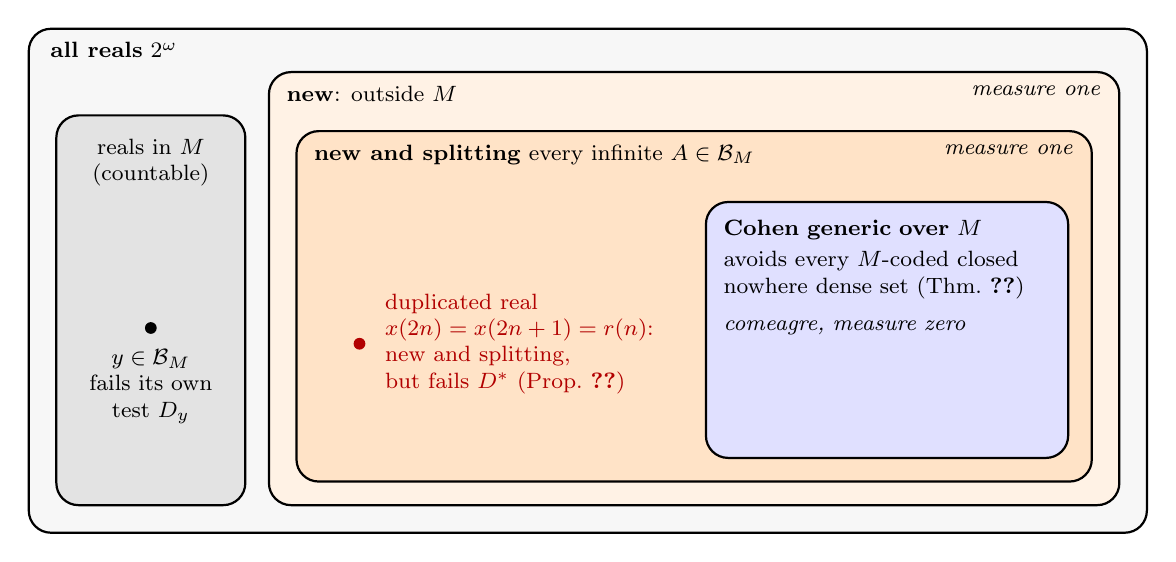
\begin{tikzpicture}[
    font=\footnotesize,
    reg/.style={draw, rounded corners=8pt, thick},
    dot/.style={circle, fill, inner sep=1.5pt}]
  % all reals
  \draw[reg, fill=gray!6] (0,0) rectangle (14.2,6.4);
  \node[anchor=north west] at (0.15,6.35) {\textbf{all reals} $2^\omega$};
  % reals in M
  \draw[reg, fill=gray!22] (0.35,0.35) rectangle (2.75,5.3);
  \node[align=center] at (1.55,4.7) {reals in $M$\\(countable)};
  \node[dot] at (1.55,2.6) {};
  \node[anchor=north, align=center] at (1.55,2.45) {$y\in\mathcal B_M$\\fails its own\\test $D_y$};
  % new reals
  \draw[reg, fill=orange!10] (3.05,0.35) rectangle (13.85,5.85);
  \node[anchor=north west] at (3.15,5.8) {\textbf{new}: outside $M$};
  \node[anchor=north east] at (13.75,5.8) {\emph{measure one}};
  % new and splitting
  \draw[reg, fill=orange!22] (3.4,0.65) rectangle (13.5,5.1);
  \node[anchor=north west] at (3.5,5.05) {\textbf{new and splitting} every infinite
    $A\in\mathcal B_M$};
  \node[anchor=north east] at (13.4,5.05) {\emph{measure one}};
  % generic
  \draw[reg, fill=blue!12] (8.6,0.95) rectangle (13.2,4.2);
  \node[anchor=north west, align=left, text width=4.3cm] at (8.7,4.1)
       {\textbf{Cohen generic over $M$}\\[2pt]avoids every $M$-coded closed nowhere
        dense set (Thm.~\ref{thm:recognition})\\[4pt]\emph{comeagre, measure zero}};
  % duplicated real
  \node[dot, red!70!black] at (4.2,2.4) {};
  \node[anchor=west, align=left, text=red!70!black] at (4.4,2.4)
       {duplicated real\\$x(2n)=x(2n+1)=r(n)$:\\new and splitting,\\but fails $D^\ast$
        (Prop.~\ref{prop:converse})};
\end{tikzpicture}
\caption{Where Cohen reals sit. Every generic real is new and splits every infinite coded set
(Theorem~\ref{thm:novelty}), so the blue region lies inside both orange ones. The converse
fails: the duplicated real (red) is new and splitting but misses the dense set $D^\ast$
(Proposition~\ref{prop:converse}). Genericity is characterized exactly by avoiding all coded closed
nowhere dense sets (Theorem~\ref{thm:recognition}). In measure the orange regions are full and the
blue region is null; in category the blue region is comeagre (Proposition~\ref{prop:category}).
Region sizes are schematic.}
\label{fig:genericity}
\end{figure}
